\documentclass[11pt]{amsart}
\usepackage{geometry}                % See geometry.pdf to learn the layout options. There are lots.
\geometry{letterpaper}                   % ... or a4paper or a5paper or ... 
%\geometry{landscape}                % Activate for for rotated page geometry
%\usepackage[parfill]{parskip}    % Activate to begin paragraphs with an empty line rather than an indent
\usepackage{graphicx}
\usepackage{amssymb}
\usepackage{epstopdf}
\usepackage{tikz}
\usetikzlibrary{3d,shapes,snakes,positioning}
\DeclareGraphicsRule{.tif}{png}{.png}{`convert #1 `dirname #1`/`basename #1 .tif`.png}

\begin{document}





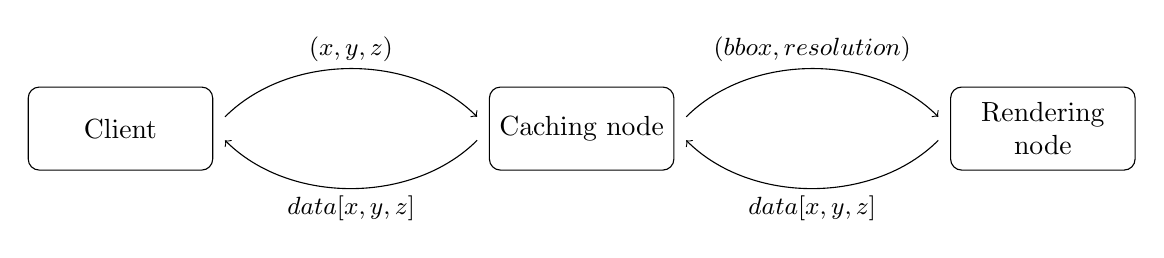
\begin{tikzpicture}[node distance=3.5cm, auto]

\tikzstyle{kasse}=[rectangle, rounded corners, draw=black, text width=6em, minimum height=3em, text centered]
\tikzstyle{pil}=[->, shorten >=6pt, shorten <=6pt]


\node[kasse] (service) {Caching node};
\node[kasse, left=of service] (client) {Client};
\node[kasse, right=of service] (data) {Rendering node};

\draw[pil, bend left=45] (client.east) to node {\small{$(x,y,z)$}} (service.west);
\draw[pil, bend left=45] (service.west) to node {\small{$data \lbrack x,y,z \rbrack$}} (client.east);
\draw[pil, bend left=45] (service.east) to node {\small{$(bbox, resolution)$}} (data.west);
\draw[pil, bend left=45] (data.west) to node {\small{$ data \lbrack x,y,z \rbrack$}} (service.east);

\end{tikzpicture}

\end{document}  